\section{Single Photon Emitters}
\label{sec:SPE}
%Bei höheren Intensitäten sollte der Dip schmaler werde, weil dann der Emitter näher an Sättigung geht und zunehmend die Lebensdauer des angeregten Zustands statt der Einstrahlphotonenrate relevant ist
%Bei 2mW angefangen zu blinken. Spektrum trotzdem gut
%Für die Spektren gegen Wellenlänge die Fläche drunter integrieren und gegen Leistung plotten

\subsection{Execution}

\begin{figure}[!ht]
    \centering
    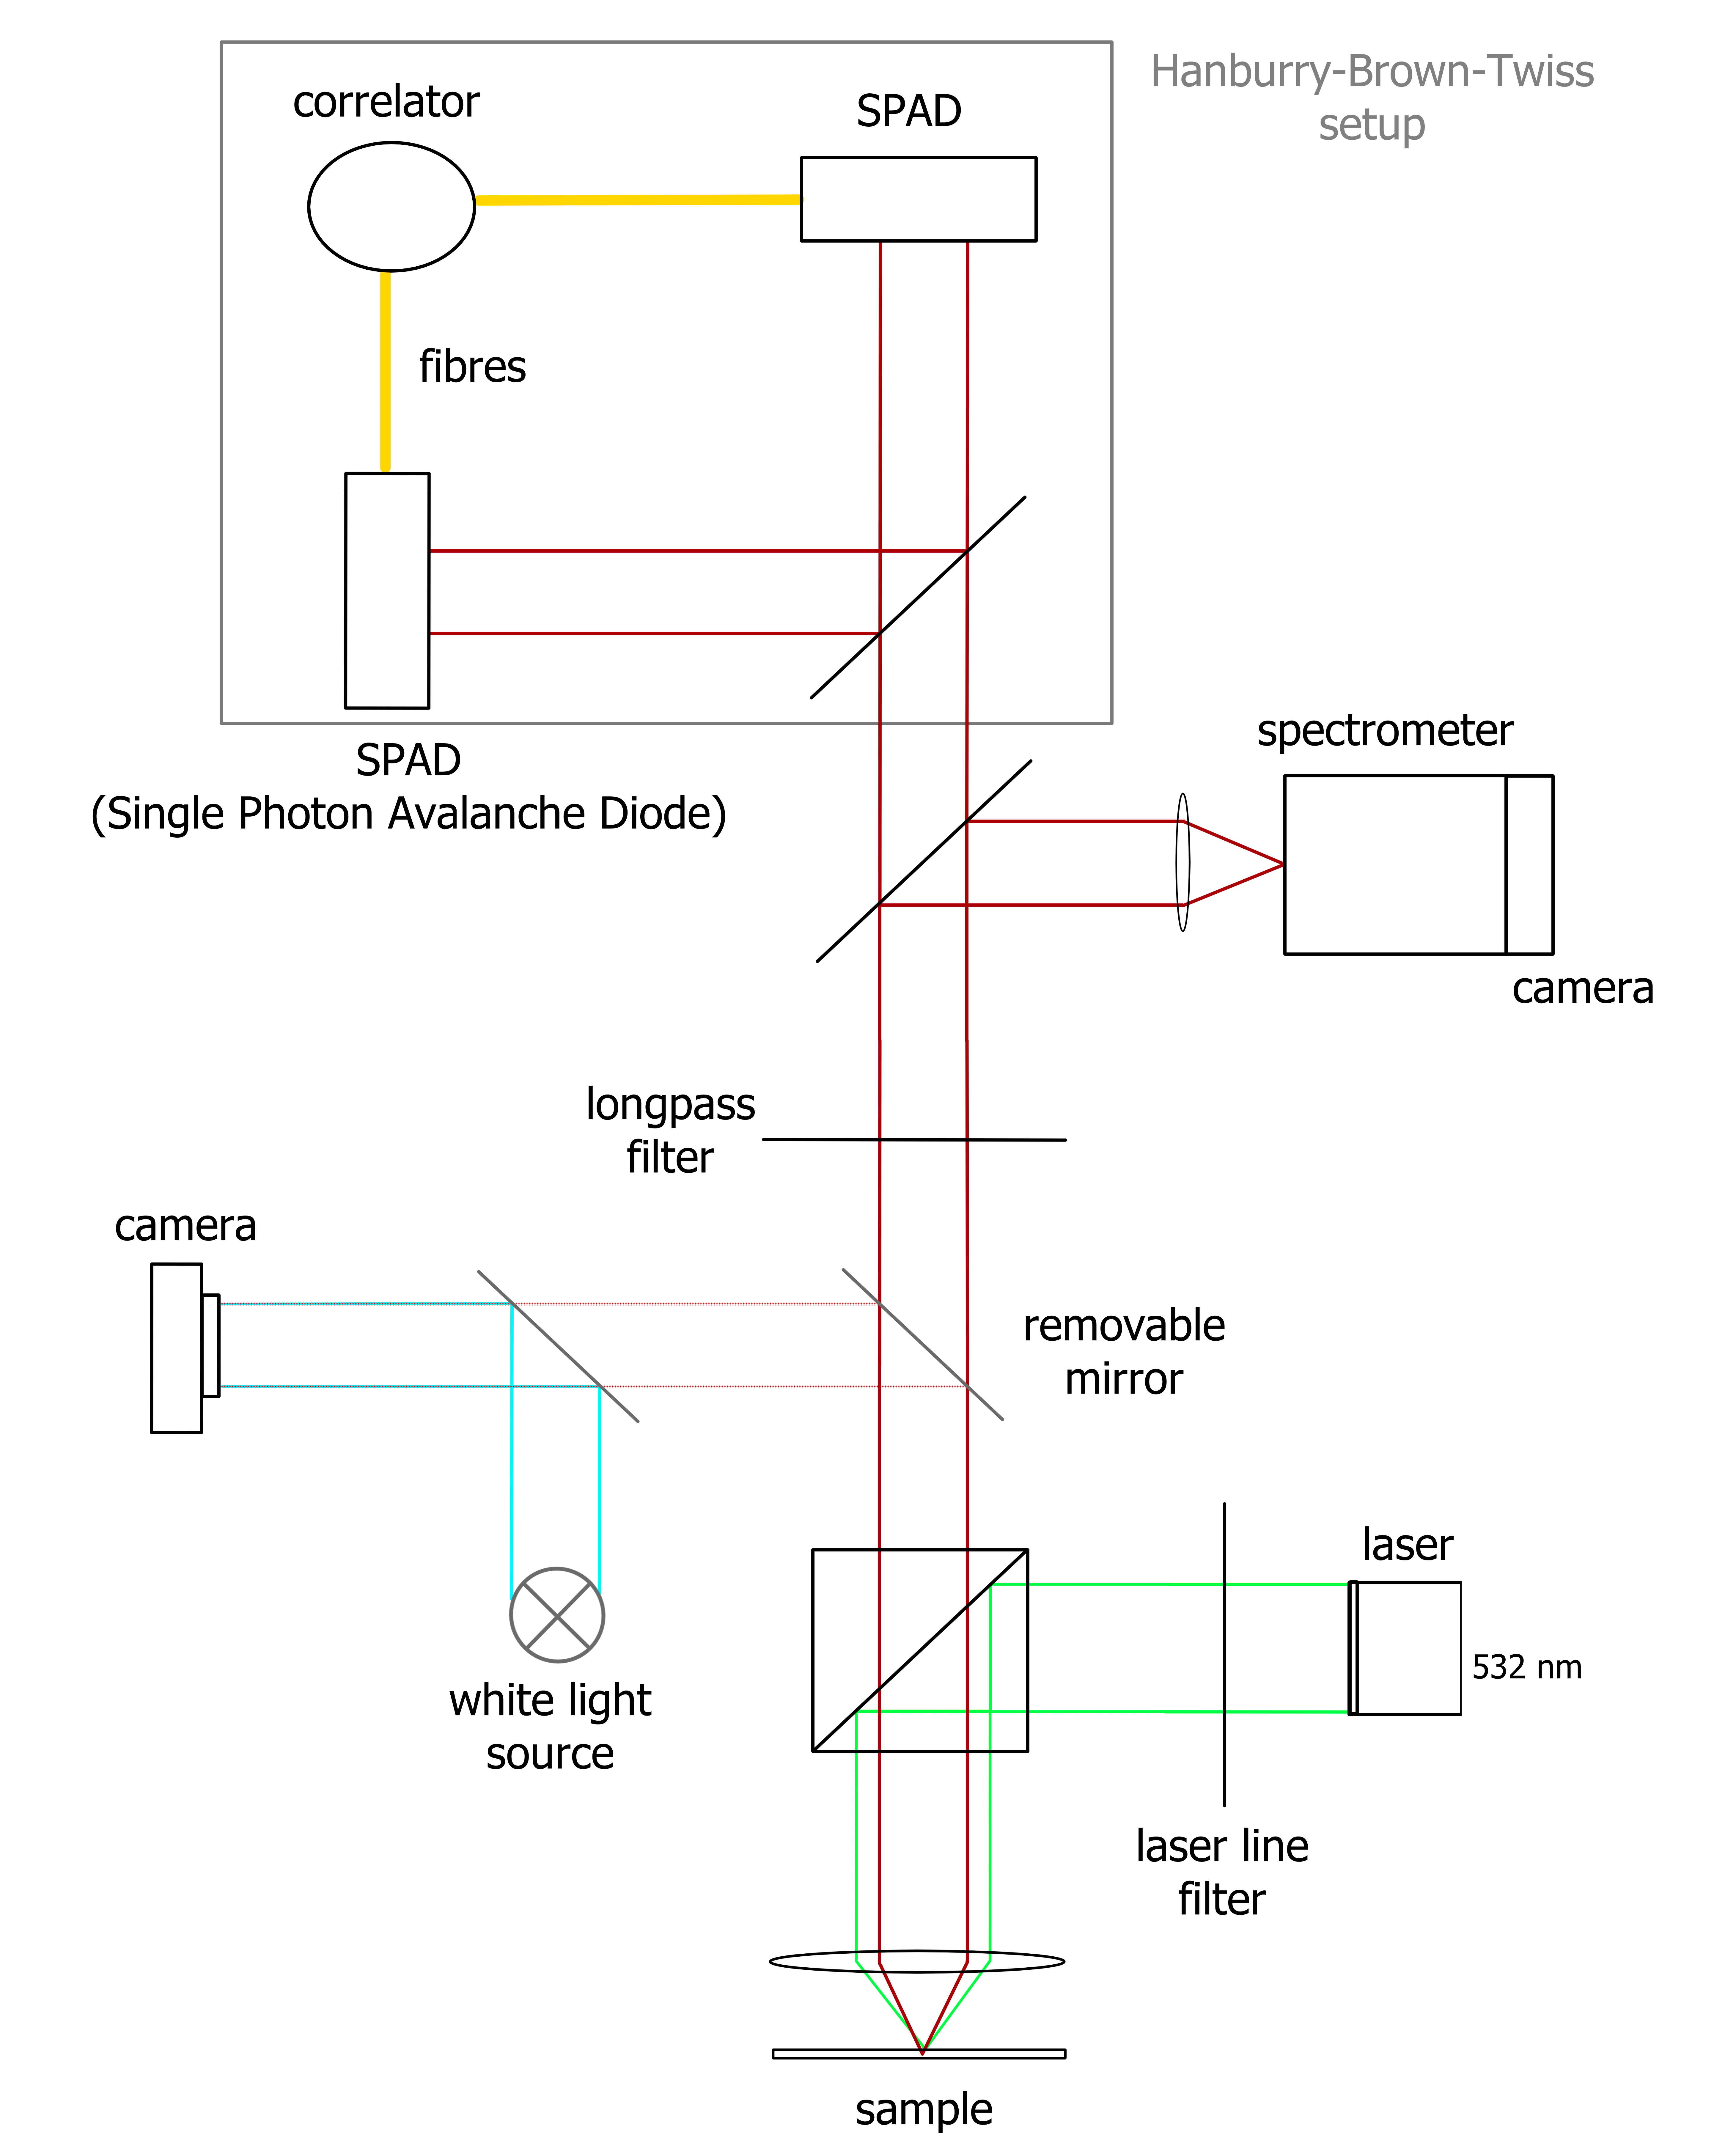
\includegraphics[width=0.7\textwidth]{img/setup2.png}
    \caption{Schematic of the confocal microscope used to record photoluminescence antibunching autocorrelation plots.}
    \label{fig_confocal}
\end{figure}

Hexagonal boron nitride powder on a substrate is viewed through a confocal microscope, which is shown in \cref{fig_confocal}.
In order to navigate on the sample, a white light source and a camera are used.
Once a promising region is found, the laser is used instead and the detector (a spectrometer) is used, to record spectra at different spots on the sample, until a single photon emitter (SPE) is found.
The SPE is identified through %TODO irgendwie, dass das Spektrum auf bestimmte Weise aussieht.

Once a suspected SPE is found, an antibunching measurement is conducted, by replacing the spectrometer with a two fibres that split the light into two parts, that are seperately measured with two detectors as described in \cref{sec:theory:spe}.
These measurements are conducted for a series of different excitation laser powers and for each measurement a seperate background measurement is done. %TODO wie wurde das background measurement gemacht? Wir haben ja nicht die Probe bewegt. Einfach Strahl direkt von Laser auf Detektor geleitet?
Additionally spectra are also recorded for increasing laser powers.

\subsection{Analysis}
\subsubsection{Antibunching}

In \cref{fig_antibunch_raw} the raw measurement data recorded in the procedure described above is shown.
In the following the measurement of the SPE will be called $S(\tau)$ and the background measurement will be called $B(\tau)$ with $\tau$ the delay measured between the two detectors.
It can be seen, that peaks exist in both measurements.
These stem from resonances in the laser, causing a not completely constant photon output rate of the laser at this small timescale.
As these resonances are independent of the sample, the background measurement contains only these resonances and can be used to derive a background corrected signal $\tilde{S} (\tau)$.
If the average number of counts in a bin far away from the dip and any resonances is $I_S$ for the SPE and $I_B$ for the background, the correction can be done as follows:
\begin{equation}
  \tilde{S} (\tau) = S - \frac{I_S}{I_B F} (B-I_B) = S - \frac{I_S}{I_B} B + I_S
\end{equation}
The factor $F$ is added artificially and maually adjusted for each measurement, as without it the resonance peaks are overestimated causing minima in the corrected signal.
In order to do this the term $\frac{I_S}{I_B F} (B-I_B) + I_S$ is plotted in comparison to the uncorrected signal as shown in \cref{fig_antibunch_background_comp} and $F$ is adjusted, until the resonance peaks match up.
In \cref{fig_antibunch_raw_corr_comp} the corrected signal $\tilde{S}$ is compared to the raw signal $S$.
Also the delay times are adjusted by an offset of \SI{98,5}{ns}, so that the dip lies at \SI{0}{ns}.
This is necessary due to slightly different travelling time of the signal between the detectors.


\begin{figure}[!ht]
    \centering
    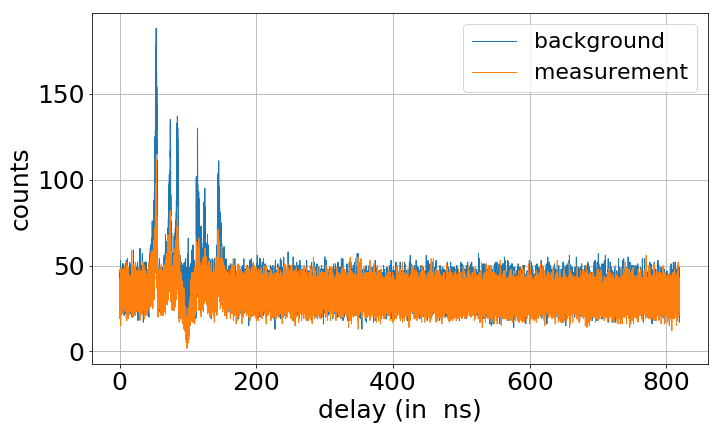
\includegraphics[width=0.7\textwidth]{img/output_t2/antibunch_example_50.0muW.png}
    \caption{Antibunching measurement as recorded. Shown is the measurement of h-BN and the pure background measurement for a laser power of \SI{50}{\micro W}.}
    \label{fig_antibunch_raw}
\end{figure}

\begin{figure}[!ht]
    \centering
    \begin{subfigure}{0.7\textwidth}
        \centering
        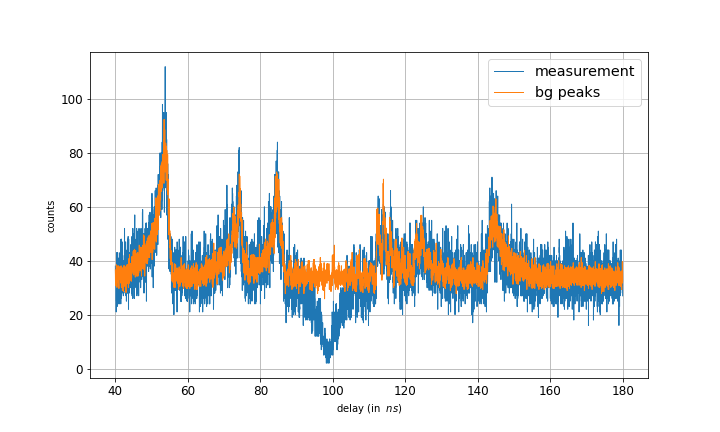
\includegraphics[width=1.0\textwidth]{img/output_t2/50.0muW_bg_peaks.png}
    \caption{}
    \label{fig_antibunch_background_comp}
    \end{subfigure}
    %\hfill
    \begin{subfigure}{0.7\textwidth}
        \centering
        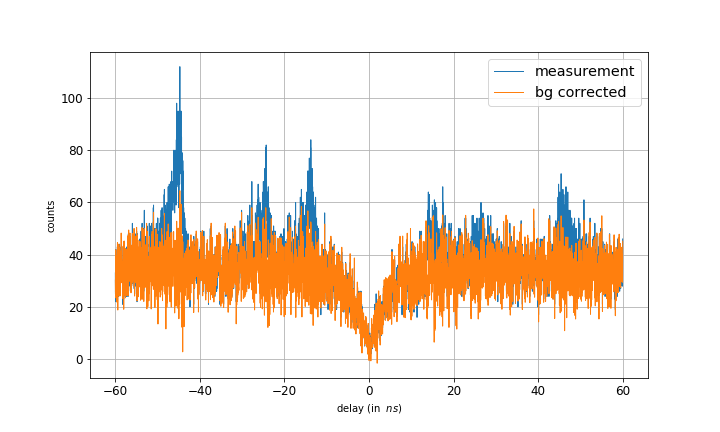
\includegraphics[width=\textwidth]{img/output_t2/50.0muW_bg_vgl.png}
        \caption{}
        \label{fig_antibunch_raw_corr_comp}
    \end{subfigure}
    \caption{a: Antibunching measurement as recorded and compared to the adjusted background signal. b: Antibunching measurement as recorded and compared to the background corrected signal. The laser power is \SI{50}{\micro W}.}
	\label{fig_antibunch_comp}
\end{figure}

This is done for six different powers and shown in \cref{sec:anhang:spe}.

These antibunching measurements show that indeed a single photon emitter was found, as they all show a large dip at a delay between start and stop signal of \SI{0}, as this means that it is at least much less likely that the source emits two photons at once, than at a finite delay.
It can also be seen, that for very high laser powers the edges of the signal start to decrease significantly with the absolute value of the delay time.
This can be explained by the fact, that here the photon rate emitted from the laser and thereby from the sample is so high that large delays between start and stop signal become increasingly unlikely.

In order to characterize the behaviour of the source at increasing excitation powers, the dip depth at the width of the dip at half of its depth is manually read from the charts.
The results are shown in \cref{fig_dip_depth} and \cref{fig_dip_width}.
The depth is normalized by $I_S$ to ensure comparibilty between measurements.
The uncertainties are gauged from the thickness of the noise.

\begin{figure}[!ht]
    \centering
    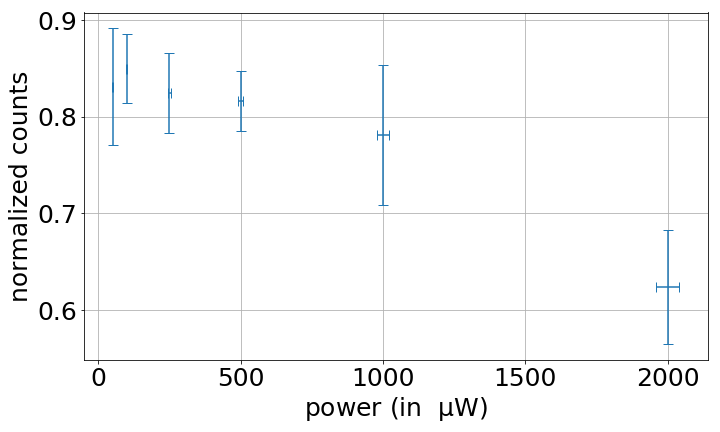
\includegraphics[width=0.7\textwidth]{img/output_t2/dip_depth.png}
    \caption{Depth of the dips in the antibunching measurements plotted against the laser power.}
    \label{fig_dip_depth}
\end{figure}

\begin{figure}[!ht]
    \centering
    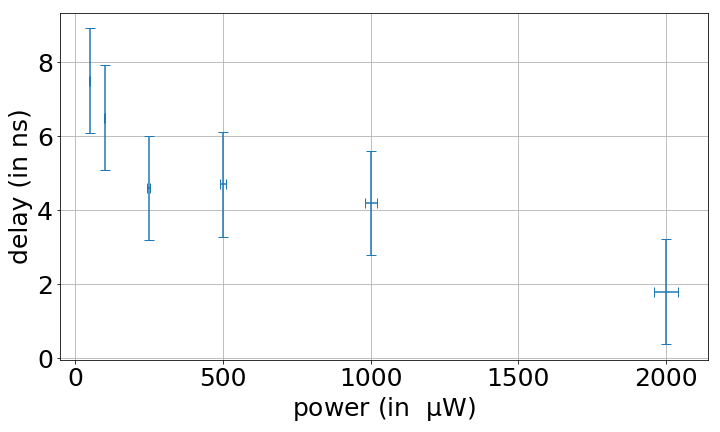
\includegraphics[width=0.7\textwidth]{img/output_t2/dip_width.png}
    \caption{Width of the dips in the antibunching measurements plotted against the laser power.}
    \label{fig_dip_width}
\end{figure}

It can be seen, that both the depth and the width decreases with increasing laser power.
For the depth this can only be explained by the increasing likelyhood that two photons hit the detectors at the same time, with at least one of them not stemming from the SPE (e.g. a reflection).
But as the width decreases at the same time, it can be seen that the emitter doesn't reach complete saturation, as in this case only the constant background would increase causing the width at half depth to increase as well.
%TODO jetzt wo ich das geschrieben habe, finde ich diese beiden Plots nicht sehr aussagevoll, da das beides ziemlich obvious ist, aber ich weiß nicht, was ich sonst mit den ganzen antibunching messungen machen soll.

%\begin{figure}[!ht]
    %\centering
    %\begin{subfigure}{0.8\textwidth}
        %\centering
        %\includegraphics[width=1.0\textwidth]{cu_stress_strain.png}
    %\caption{Measurement.}
    %\label{cu_stress_strain}
    %\end{subfigure}
    %%\hfill
    %\begin{subfigure}{0.8\textwidth}
        %\centering
        %\includegraphics[width=\textwidth]{shabnam_technical-stress-strain.png}
        %\caption{Reference.}
        %\label{fig_shabnam_tss}
    %\end{subfigure}
    %\caption{Technical stress-strain-curve of a copper single crystal and reference provided by the instructor.}
	%\label{cu_stress_strain_ges}
%\end{figure}

\subsubsection{Power efficiency of the SPE}
